\documentclass[12pt]{article}
\usepackage[utf8]{inputenc}
\usepackage[french]{babel}
\usepackage{graphicx} % Required for inserting images
\usepackage[export]{adjustbox}
\usepackage[margin=1cm]{cmpt}
\usepackage{xcolor}
\usepackage{tikz}
\usepackage{float}
\usepackage{pgfplots}
\usepackage{amssymb}
\usepackage{amsmath}
\usepackage[most]{tcolorbox}
\usepackage{lmodern}
\usepackage{amsmath}
\usepackage{caption}
\usepackage[normalem]{ulem}
\usepackage{tabularx}
\usetikzlibrary{
    matrix,
    arrows.meta,
    automata, 
    arrows,
    positioning,
    shapes.geometric,
    shapes.arrows,
    patterns,
    fit,
    shapes.geometric,
    calc
}

\setlength{\parindent}{0em}

\definecolor{custombordercolor}{RGB}{213,84,84}
\definecolor{myblue}{rgb}{0.6,0.8,1} % Définir la couleur bleu clair avec RVB
\definecolor{bluetitle}{HTML}{99ccff}

\newcommand{\encircle}[1]{%
  \tikz[baseline=(X.base)]
    \node (X) [draw, shape=circle, inner sep=0pt] {\strut
#1};%
}


\begin{document}
%Q
Quel principe fondamental existe-t-il pour les composants graphiques en Java~?
%R

Toute manipulation (directe ou indirecte) d'un composant graphique doit se
faire sur le thread graphique (EDT).
%F

\vphantom{}

%Q
Qu'est-ce qu'est l'\textbf{EDT}~?
%R

Il s'agit de l'\textbf{Event Dispatch Thread}.

\begin{itemize}
  \item thread dédié à la gestion des composants graphiques
  \item accède aux événements graphiques par une \code{EventQueue}
\end{itemize}
%F

\vphantom{}

%Q
Donner le principe de gestion de l'interaction des composants graphiques avec
l'utilisateur.
%R

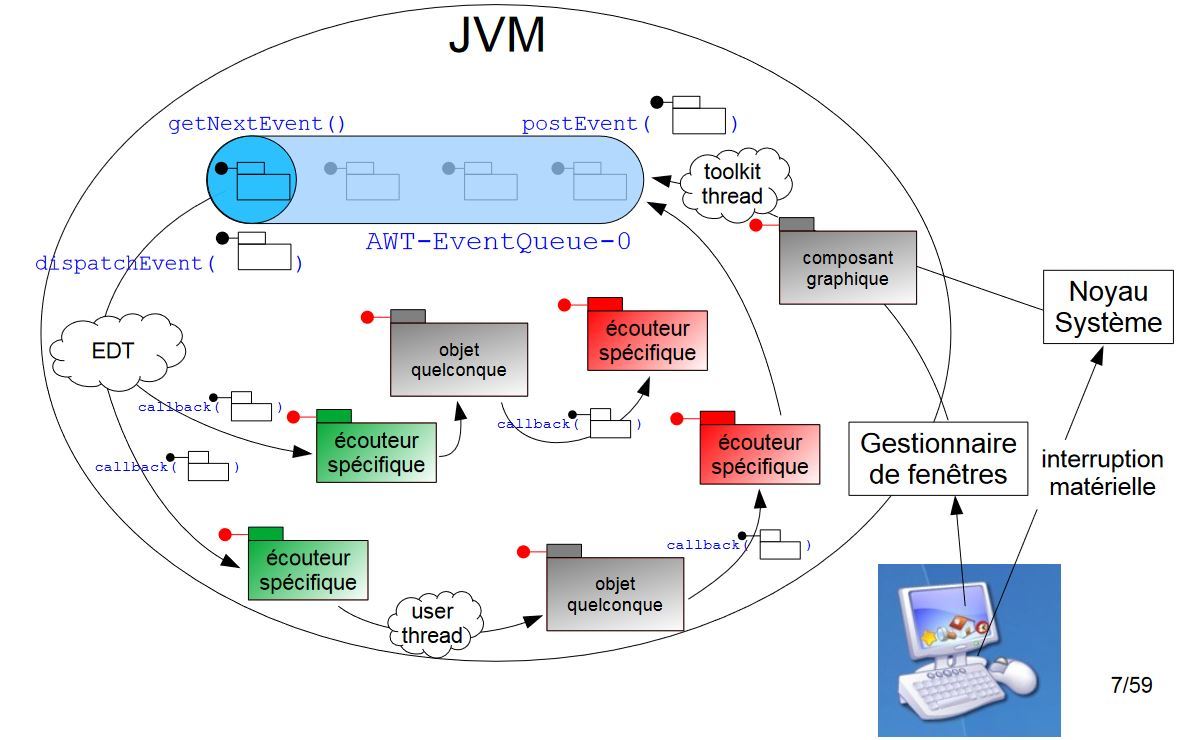
\includegraphics[scale=.7]{img/mpoo/idee_graphique.JPG}
%F

\vphantom{}

\end{document}